\documentclass[1p]{elsarticle_modified}
%\bibliographystyle{elsarticle-num}

%\usepackage[colorlinks]{hyperref}
%\usepackage{abbrmath_seonhwa} %\Abb, \Ascr, \Acal ,\Abf, \Afrak
\usepackage{amsfonts}
\usepackage{amssymb}
\usepackage{amsmath}
\usepackage{amsthm}
\usepackage{scalefnt}
\usepackage{amsbsy}
\usepackage{kotex}
\usepackage{caption}
\usepackage{subfig}
\usepackage{color}
\usepackage{graphicx}
\usepackage{xcolor} %% white, black, red, green, blue, cyan, magenta, yellow
\usepackage{float}
\usepackage{setspace}
\usepackage{hyperref}

\usepackage{tikz}
\usetikzlibrary{arrows}

\usepackage{multirow}
\usepackage{array} % fixed length table
\usepackage{hhline}

%%%%%%%%%%%%%%%%%%%%%
\makeatletter
\renewcommand*\env@matrix[1][\arraystretch]{%
	\edef\arraystretch{#1}%
	\hskip -\arraycolsep
	\let\@ifnextchar\new@ifnextchar
	\array{*\c@MaxMatrixCols c}}
\makeatother %https://tex.stackexchange.com/questions/14071/how-can-i-increase-the-line-spacing-in-a-matrix
%%%%%%%%%%%%%%%

\usepackage[normalem]{ulem}

\newcommand{\msout}[1]{\ifmmode\text{\sout{\ensuremath{#1}}}\else\sout{#1}\fi}
%SOURCE: \msout is \stkout macro in https://tex.stackexchange.com/questions/20609/strikeout-in-math-mode

\newcommand{\cancel}[1]{
	\ifmmode
	{\color{red}\msout{#1}}
	\else
	{\color{red}\sout{#1}}
	\fi
}

\newcommand{\add}[1]{
	{\color{blue}\uwave{#1}}
}

\newcommand{\replace}[2]{
	\ifmmode
	{\color{red}\msout{#1}}{\color{blue}\uwave{#2}}
	\else
	{\color{red}\sout{#1}}{\color{blue}\uwave{#2}}
	\fi
}

\newcommand{\Sol}{\mathcal{S}} %segment
\newcommand{\D}{D} %diagram
\newcommand{\A}{\mathcal{A}} %arc


%%%%%%%%%%%%%%%%%%%%%%%%%%%%%5 test

\def\sl{\operatorname{\textup{SL}}(2,\Cbb)}
\def\psl{\operatorname{\textup{PSL}}(2,\Cbb)}
\def\quan{\mkern 1mu \triangleright \mkern 1mu}

\theoremstyle{definition}
\newtheorem{thm}{Theorem}[section]
\newtheorem{prop}[thm]{Proposition}
\newtheorem{lem}[thm]{Lemma}
\newtheorem{ques}[thm]{Question}
\newtheorem{cor}[thm]{Corollary}
\newtheorem{defn}[thm]{Definition}
\newtheorem{exam}[thm]{Example}
\newtheorem{rmk}[thm]{Remark}
\newtheorem{alg}[thm]{Algorithm}

\newcommand{\I}{\sqrt{-1}}
\begin{document}

%\begin{frontmatter}
%
%\title{Boundary parabolic representations of knots up to 8 crossings}
%
%%% Group authors per affiliation:
%\author{Yunhi Cho} 
%\address{Department of Mathematics, University of Seoul, Seoul, Korea}
%\ead{yhcho@uos.ac.kr}
%
%
%\author{Seonhwa Kim} %\fnref{s_kim}}
%\address{Center for Geometry and Physics, Institute for Basic Science, Pohang, 37673, Korea}
%\ead{ryeona17@ibs.re.kr}
%
%\author{Hyuk Kim}
%\address{Department of Mathematical Sciences, Seoul National University, Seoul 08826, Korea}
%\ead{hyukkim@snu.ac.kr}
%
%\author{Seokbeom Yoon}
%\address{Department of Mathematical Sciences, Seoul National University, Seoul, 08826,  Korea}
%\ead{sbyoon15@snu.ac.kr}
%
%\begin{abstract}
%We find all boundary parabolic representation of knots up to 8 crossings.
%
%\end{abstract}
%\begin{keyword}
%    \MSC[2010] 57M25 
%\end{keyword}
%
%\end{frontmatter}

%\linenumbers
%\tableofcontents
%
\newcommand\colored[1]{\textcolor{white}{\rule[-0.35ex]{0.8em}{1.4ex}}\kern-0.8em\color{red} #1}%
%\newcommand\colored[1]{\textcolor{white}{ #1}\kern-2.17ex	\textcolor{white}{ #1}\kern-1.81ex	\textcolor{white}{ #1}\kern-2.15ex\color{red}#1	}

{\Large $\underline{12a_{0130}~(K12a_{0130})}$}

\setlength{\tabcolsep}{10pt}
\renewcommand{\arraystretch}{1.6}
\vspace{1cm}\begin{tabular}{m{100pt}>{\centering\arraybackslash}m{274pt}}
\multirow{5}{120pt}{
	\centering
	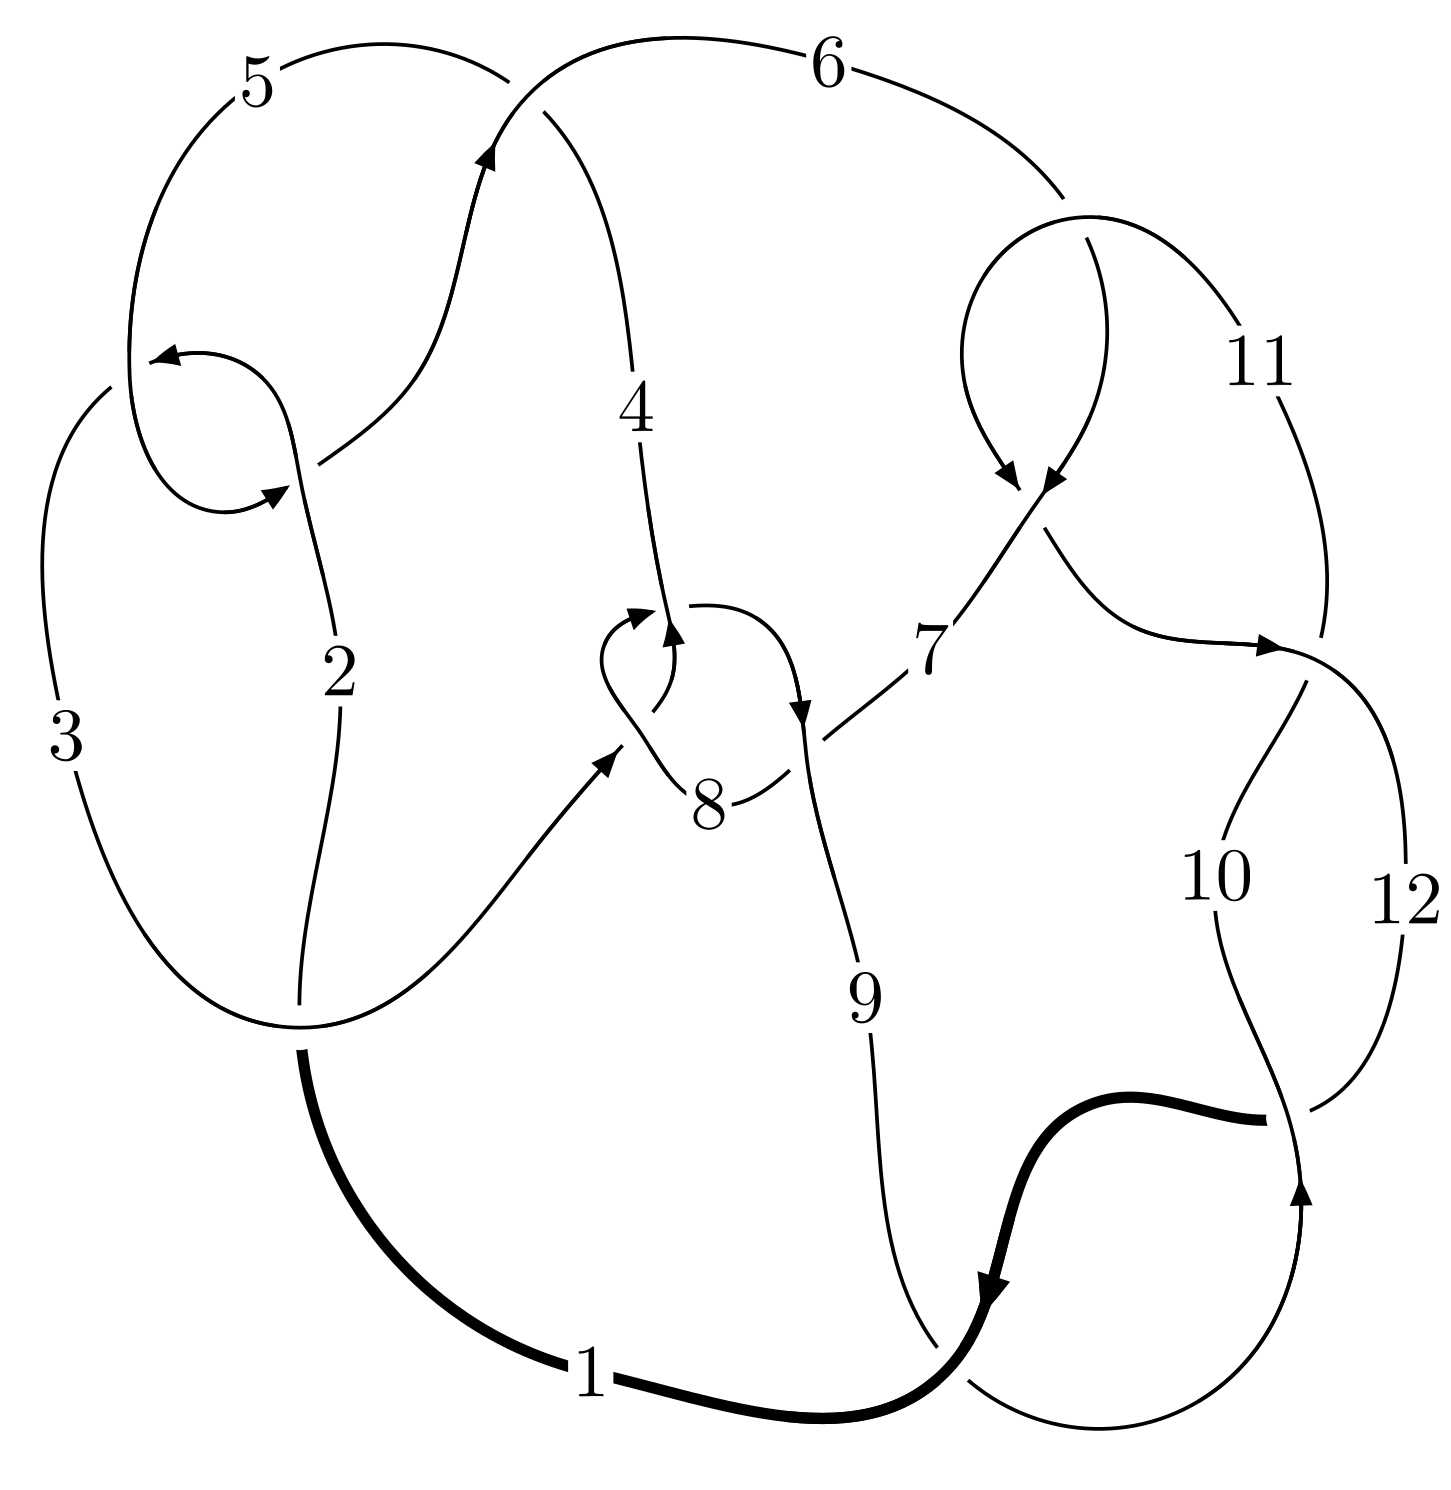
\includegraphics[width=112pt]{../../../GIT/diagram.site/Diagrams/png/931_12a_0130.png}\\
\ \ \ A knot diagram\footnotemark}&
\allowdisplaybreaks
\textbf{Linearized knot diagam} \\
\cline{2-2}
 &
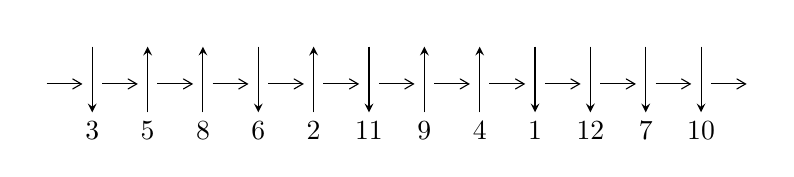
\begin{tikzpicture}[x=20pt, y=17pt]
	% nodes
	\node (C0) at (0, 0) {};
	\node (C1) at (1, 0) {};
	\node (C1U) at (1, +1) {};
	\node (C1D) at (1, -1) {3};

	\node (C2) at (2, 0) {};
	\node (C2U) at (2, +1) {};
	\node (C2D) at (2, -1) {5};

	\node (C3) at (3, 0) {};
	\node (C3U) at (3, +1) {};
	\node (C3D) at (3, -1) {8};

	\node (C4) at (4, 0) {};
	\node (C4U) at (4, +1) {};
	\node (C4D) at (4, -1) {6};

	\node (C5) at (5, 0) {};
	\node (C5U) at (5, +1) {};
	\node (C5D) at (5, -1) {2};

	\node (C6) at (6, 0) {};
	\node (C6U) at (6, +1) {};
	\node (C6D) at (6, -1) {11};

	\node (C7) at (7, 0) {};
	\node (C7U) at (7, +1) {};
	\node (C7D) at (7, -1) {9};

	\node (C8) at (8, 0) {};
	\node (C8U) at (8, +1) {};
	\node (C8D) at (8, -1) {4};

	\node (C9) at (9, 0) {};
	\node (C9U) at (9, +1) {};
	\node (C9D) at (9, -1) {1};

	\node (C10) at (10, 0) {};
	\node (C10U) at (10, +1) {};
	\node (C10D) at (10, -1) {12};

	\node (C11) at (11, 0) {};
	\node (C11U) at (11, +1) {};
	\node (C11D) at (11, -1) {7};

	\node (C12) at (12, 0) {};
	\node (C12U) at (12, +1) {};
	\node (C12D) at (12, -1) {10};
	\node (C13) at (13, 0) {};

	% arrows
	\draw[->,>={angle 60}]
	(C0) edge (C1) (C1) edge (C2) (C2) edge (C3) (C3) edge (C4) (C4) edge (C5) (C5) edge (C6) (C6) edge (C7) (C7) edge (C8) (C8) edge (C9) (C9) edge (C10) (C10) edge (C11) (C11) edge (C12) (C12) edge (C13) ;	\draw[->,>=stealth]
	(C1U) edge (C1D) (C2D) edge (C2U) (C3D) edge (C3U) (C4U) edge (C4D) (C5D) edge (C5U) (C6U) edge (C6D) (C7D) edge (C7U) (C8D) edge (C8U) (C9U) edge (C9D) (C10U) edge (C10D) (C11U) edge (C11D) (C12U) edge (C12D) ;
	\end{tikzpicture} \\
\hhline{~~} \\& 
\textbf{Solving Sequence} \\ \cline{2-2} 
 &
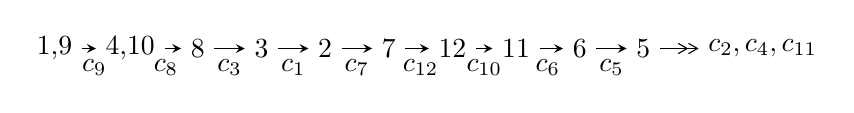
\begin{tikzpicture}[x=23pt, y=7pt]
	% node
	\node (A0) at (-1/8, 0) {1,9};
	\node (A1) at (17/16, 0) {4,10};
	\node (A2) at (17/8, 0) {8};
	\node (A3) at (25/8, 0) {3};
	\node (A4) at (33/8, 0) {2};
	\node (A5) at (41/8, 0) {7};
	\node (A6) at (49/8, 0) {12};
	\node (A7) at (57/8, 0) {11};
	\node (A8) at (65/8, 0) {6};
	\node (A9) at (73/8, 0) {5};
	\node (C1) at (1/2, -1) {$c_{9}$};
	\node (C2) at (13/8, -1) {$c_{8}$};
	\node (C3) at (21/8, -1) {$c_{3}$};
	\node (C4) at (29/8, -1) {$c_{1}$};
	\node (C5) at (37/8, -1) {$c_{7}$};
	\node (C6) at (45/8, -1) {$c_{12}$};
	\node (C7) at (53/8, -1) {$c_{10}$};
	\node (C8) at (61/8, -1) {$c_{6}$};
	\node (C9) at (69/8, -1) {$c_{5}$};
	\node (A10) at (11, 0) {$c_{2},c_{4},c_{11}$};

	% edge
	\draw[->,>=stealth]	
	(A0) edge (A1) (A1) edge (A2) (A2) edge (A3) (A3) edge (A4) (A4) edge (A5) (A5) edge (A6) (A6) edge (A7) (A7) edge (A8) (A8) edge (A9) ;
	\draw[->>,>={angle 60}]	
	(A9) edge (A10);
\end{tikzpicture} \\ 

\end{tabular} \\

\footnotetext{
The image of knot diagram is generated by the software ``\textbf{Draw programme}" developed by Andrew Bartholomew(\url{http://www.layer8.co.uk/maths/draw/index.htm\#Running-draw}), where we modified some parts for our purpose(\url{https://github.com/CATsTAILs/LinksPainter}).
}\phantom \\ \newline 
\centering \textbf{Ideals for irreducible components\footnotemark of $X_{\text{par}}$} 
 
\begin{align*}
I^u_{1}&=\langle 
1.71551\times10^{48} u^{81}-3.44735\times10^{49} u^{80}+\cdots+8.87210\times10^{48} b+2.83258\times10^{48},\\
\phantom{I^u_{1}}&\phantom{= \langle  }2.41231\times10^{48} u^{81}-5.91476\times10^{49} u^{80}+\cdots+1.77442\times10^{49} a-5.95155\times10^{49},\;u^{82}-21 u^{81}+\cdots-6 u+1\rangle \\
I^u_{2}&=\langle 
b,\;u^2 a+a^2- a u+2 u^2+2 a- u+3,\;u^3- u^2+2 u-1\rangle \\
\\
\end{align*}
\raggedright * 2 irreducible components of $\dim_{\mathbb{C}}=0$, with total 88 representations.\\
\footnotetext{All coefficients of polynomials are rational numbers. But the coefficients are sometimes approximated in decimal forms when there is not enough margin.}
\newpage
\renewcommand{\arraystretch}{1}
\centering \section*{I. $I^u_{1}= \langle 1.72\times10^{48} u^{81}-3.45\times10^{49} u^{80}+\cdots+8.87\times10^{48} b+2.83\times10^{48},\;2.41\times10^{48} u^{81}-5.91\times10^{49} u^{80}+\cdots+1.77\times10^{49} a-5.95\times10^{49},\;u^{82}-21 u^{81}+\cdots-6 u+1 \rangle$}
\flushleft \textbf{(i) Arc colorings}\\
\begin{tabular}{m{7pt} m{180pt} m{7pt} m{180pt} }
\flushright $a_{1}=$&$\begin{pmatrix}0\\u\end{pmatrix}$ \\
\flushright $a_{9}=$&$\begin{pmatrix}1\\0\end{pmatrix}$ \\
\flushright $a_{4}=$&$\begin{pmatrix}-0.135949 u^{81}+3.33335 u^{80}+\cdots-14.6043 u+3.35408\\-0.193360 u^{81}+3.88560 u^{80}+\cdots-1.25258 u-0.319268\end{pmatrix}$ \\
\flushright $a_{10}=$&$\begin{pmatrix}1\\u^2\end{pmatrix}$ \\
\flushright $a_{8}=$&$\begin{pmatrix}0.279029 u^{81}-5.76662 u^{80}+\cdots-2.69338 u-0.263304\\0.124157 u^{81}-2.30644 u^{80}+\cdots+0.756435 u-0.180204\end{pmatrix}$ \\
\flushright $a_{3}=$&$\begin{pmatrix}0.423190 u^{81}-8.54849 u^{80}+\cdots-15.2890 u+3.49093\\0.112206 u^{81}-2.46762 u^{80}+\cdots-4.37396 u+0.0898841\end{pmatrix}$ \\
\flushright $a_{2}=$&$\begin{pmatrix}-1.77927 u^{81}+36.7421 u^{80}+\cdots-25.6185 u+3.03635\\-0.339356 u^{81}+7.17752 u^{80}+\cdots-1.91577 u+0.353373\end{pmatrix}$ \\
\flushright $a_{7}=$&$\begin{pmatrix}0.154872 u^{81}-3.46018 u^{80}+\cdots-3.44981 u-0.0831007\\0.124157 u^{81}-2.30644 u^{80}+\cdots+0.756435 u-0.180204\end{pmatrix}$ \\
\flushright $a_{12}=$&$\begin{pmatrix}u\\u^3+u\end{pmatrix}$ \\
\flushright $a_{11}=$&$\begin{pmatrix}u^2+1\\u^4+2 u^2\end{pmatrix}$ \\
\flushright $a_{6}=$&$\begin{pmatrix}-0.180204 u^{81}+3.66012 u^{80}+\cdots-5.94908 u+0.324786\\-0.0929984 u^{81}+2.05540 u^{80}+\cdots-1.41087 u+0.279029\end{pmatrix}$ \\
\flushright $a_{5}=$&$\begin{pmatrix}0.347186 u^{81}-7.10288 u^{80}+\cdots-17.9030 u+3.60140\\0.0229512 u^{81}-0.648699 u^{80}+\cdots-3.43429 u-0.230274\end{pmatrix}$\\&\end{tabular}
\flushleft \textbf{(ii) Obstruction class $= -1$}\\~\\
\flushleft \textbf{(iii) Cusp Shapes $= 6.00126 u^{81}-124.839 u^{80}+\cdots+77.6881 u-11.3348$}\\~\\
\newpage\renewcommand{\arraystretch}{1}
\flushleft \textbf{(iv) u-Polynomials at the component}\newline \\
\begin{tabular}{m{50pt}|m{274pt}}
Crossings & \hspace{64pt}u-Polynomials at each crossing \\
\hline $$\begin{aligned}c_{1},c_{4}\end{aligned}$$&$\begin{aligned}
&u^{82}+28 u^{81}+\cdots+17 u+1
\end{aligned}$\\
\hline $$\begin{aligned}c_{2},c_{5}\end{aligned}$$&$\begin{aligned}
&u^{82}+4 u^{81}+\cdots+u+1
\end{aligned}$\\
\hline $$\begin{aligned}c_{3},c_{8}\end{aligned}$$&$\begin{aligned}
&u^{82}- u^{81}+\cdots+224 u+64
\end{aligned}$\\
\hline $$\begin{aligned}c_{6},c_{11}\end{aligned}$$&$\begin{aligned}
&u^{82}+3 u^{81}+\cdots-3 u^2+1
\end{aligned}$\\
\hline $$\begin{aligned}c_{7}\end{aligned}$$&$\begin{aligned}
&u^{82}-35 u^{81}+\cdots-62464 u+4096
\end{aligned}$\\
\hline $$\begin{aligned}c_{9},c_{10},c_{12}\end{aligned}$$&$\begin{aligned}
&u^{82}+21 u^{81}+\cdots+6 u+1
\end{aligned}$\\
\hline
\end{tabular}\\~\\
\newpage\renewcommand{\arraystretch}{1}
\flushleft \textbf{(v) Riley Polynomials at the component}\newline \\
\begin{tabular}{m{50pt}|m{274pt}}
Crossings & \hspace{64pt}Riley Polynomials at each crossing \\
\hline $$\begin{aligned}c_{1},c_{4}\end{aligned}$$&$\begin{aligned}
&y^{82}+56 y^{81}+\cdots-247 y+1
\end{aligned}$\\
\hline $$\begin{aligned}c_{2},c_{5}\end{aligned}$$&$\begin{aligned}
&y^{82}+28 y^{81}+\cdots+17 y+1
\end{aligned}$\\
\hline $$\begin{aligned}c_{3},c_{8}\end{aligned}$$&$\begin{aligned}
&y^{82}-35 y^{81}+\cdots-62464 y+4096
\end{aligned}$\\
\hline $$\begin{aligned}c_{6},c_{11}\end{aligned}$$&$\begin{aligned}
&y^{82}-21 y^{81}+\cdots-6 y+1
\end{aligned}$\\
\hline $$\begin{aligned}c_{7}\end{aligned}$$&$\begin{aligned}
&y^{82}+13 y^{81}+\cdots+200278016 y+16777216
\end{aligned}$\\
\hline $$\begin{aligned}c_{9},c_{10},c_{12}\end{aligned}$$&$\begin{aligned}
&y^{82}+83 y^{81}+\cdots+34 y+1
\end{aligned}$\\
\hline
\end{tabular}\\~\\
\newpage\flushleft \textbf{(vi) Complex Volumes and Cusp Shapes}
$$\begin{array}{c|c|c}  
\text{Solutions to }I^u_{1}& \I (\text{vol} + \sqrt{-1}CS) & \text{Cusp shape}\\
 \hline 
\begin{aligned}
u &= \phantom{-}0.966335 + 0.246919 I \\
a &= -0.915807 - 0.552310 I \\
b &= -0.932256 - 0.420934 I\end{aligned}
 & -0.0961212 - 0.0220843 I & \phantom{-0.000000 } 0 \\ \hline\begin{aligned}
u &= \phantom{-}0.966335 - 0.246919 I \\
a &= -0.915807 + 0.552310 I \\
b &= -0.932256 + 0.420934 I\end{aligned}
 & -0.0961212 + 0.0220843 I & \phantom{-0.000000 } 0 \\ \hline\begin{aligned}
u &= \phantom{-}0.868429 + 0.444440 I \\
a &= \phantom{-}0.686912 + 0.981827 I \\
b &= \phantom{-}0.754394 + 0.707664 I\end{aligned}
 & -5.26651 - 0.17540 I & \phantom{-0.000000 } 0 \\ \hline\begin{aligned}
u &= \phantom{-}0.868429 - 0.444440 I \\
a &= \phantom{-}0.686912 - 0.981827 I \\
b &= \phantom{-}0.754394 - 0.707664 I\end{aligned}
 & -5.26651 + 0.17540 I & \phantom{-0.000000 } 0 \\ \hline\begin{aligned}
u &= \phantom{-}0.835016 + 0.604230 I \\
a &= -0.11512 - 1.66139 I \\
b &= \phantom{-}0.906919 - 0.662661 I\end{aligned}
 & -4.79650 - 5.41790 I & \phantom{-0.000000 } 0 \\ \hline\begin{aligned}
u &= \phantom{-}0.835016 - 0.604230 I \\
a &= -0.11512 + 1.66139 I \\
b &= \phantom{-}0.906919 + 0.662661 I\end{aligned}
 & -4.79650 + 5.41790 I & \phantom{-0.000000 } 0 \\ \hline\begin{aligned}
u &= \phantom{-}0.735295 + 0.603136 I \\
a &= \phantom{-}0.401497 + 1.324250 I \\
b &= \phantom{-}0.548094 + 0.869830 I\end{aligned}
 & -1.46626 - 5.79986 I & \phantom{-0.000000 } 0 \\ \hline\begin{aligned}
u &= \phantom{-}0.735295 - 0.603136 I \\
a &= \phantom{-}0.401497 - 1.324250 I \\
b &= \phantom{-}0.548094 - 0.869830 I\end{aligned}
 & -1.46626 + 5.79986 I & \phantom{-0.000000 } 0 \\ \hline\begin{aligned}
u &= \phantom{-}1.003680 + 0.315252 I \\
a &= \phantom{-}0.993929 + 0.707315 I \\
b &= \phantom{-}0.984089 + 0.537506 I\end{aligned}
 & -0.98184 + 5.34647 I & \phantom{-0.000000 } 0 \\ \hline\begin{aligned}
u &= \phantom{-}1.003680 - 0.315252 I \\
a &= \phantom{-}0.993929 - 0.707315 I \\
b &= \phantom{-}0.984089 - 0.537506 I\end{aligned}
 & -0.98184 - 5.34647 I & \phantom{-0.000000 } 0\\
 \hline 
 \end{array}$$\newpage$$\begin{array}{c|c|c}  
\text{Solutions to }I^u_{1}& \I (\text{vol} + \sqrt{-1}CS) & \text{Cusp shape}\\
 \hline 
\begin{aligned}
u &= \phantom{-}0.658324 + 0.598113 I \\
a &= \phantom{-}0.485356 + 1.246000 I \\
b &= -0.843150 + 0.470953 I\end{aligned}
 & -0.30459 - 3.53700 I & \phantom{-0.000000 } 0 \\ \hline\begin{aligned}
u &= \phantom{-}0.658324 - 0.598113 I \\
a &= \phantom{-}0.485356 - 1.246000 I \\
b &= -0.843150 - 0.470953 I\end{aligned}
 & -0.30459 + 3.53700 I & \phantom{-0.000000 } 0 \\ \hline\begin{aligned}
u &= -0.117177 + 0.876232 I \\
a &= -0.486743 - 0.492557 I \\
b &= -1.077990 + 0.309869 I\end{aligned}
 & \phantom{-}4.85512 - 5.44738 I & \phantom{-0.000000 } 0 \\ \hline\begin{aligned}
u &= -0.117177 - 0.876232 I \\
a &= -0.486743 + 0.492557 I \\
b &= -1.077990 - 0.309869 I\end{aligned}
 & \phantom{-}4.85512 + 5.44738 I & \phantom{-0.000000 } 0 \\ \hline\begin{aligned}
u &= \phantom{-}0.838027 + 0.747480 I \\
a &= -0.18699 + 1.40186 I \\
b &= -1.077520 + 0.593293 I\end{aligned}
 & \phantom{-}1.35820 - 5.83610 I & \phantom{-0.000000 } 0 \\ \hline\begin{aligned}
u &= \phantom{-}0.838027 - 0.747480 I \\
a &= -0.18699 - 1.40186 I \\
b &= -1.077520 - 0.593293 I\end{aligned}
 & \phantom{-}1.35820 + 5.83610 I & \phantom{-0.000000 } 0 \\ \hline\begin{aligned}
u &= \phantom{-}0.887691 + 0.734910 I \\
a &= \phantom{-}0.24737 - 1.52308 I \\
b &= \phantom{-}1.093880 - 0.659857 I\end{aligned}
 & \phantom{-}0.24237 - 11.48170 I & \phantom{-0.000000 } 0 \\ \hline\begin{aligned}
u &= \phantom{-}0.887691 - 0.734910 I \\
a &= \phantom{-}0.24737 + 1.52308 I \\
b &= \phantom{-}1.093880 + 0.659857 I\end{aligned}
 & \phantom{-}0.24237 + 11.48170 I & \phantom{-0.000000 } 0 \\ \hline\begin{aligned}
u &= \phantom{-}0.635956 + 0.545968 I \\
a &= -0.179327 - 1.211200 I \\
b &= -0.459141 - 0.788281 I\end{aligned}
 & -0.506279 - 0.677239 I & \phantom{-0.000000 } 0 \\ \hline\begin{aligned}
u &= \phantom{-}0.635956 - 0.545968 I \\
a &= -0.179327 + 1.211200 I \\
b &= -0.459141 + 0.788281 I\end{aligned}
 & -0.506279 + 0.677239 I & \phantom{-0.000000 } 0\\
 \hline 
 \end{array}$$\newpage$$\begin{array}{c|c|c}  
\text{Solutions to }I^u_{1}& \I (\text{vol} + \sqrt{-1}CS) & \text{Cusp shape}\\
 \hline 
\begin{aligned}
u &= \phantom{-}0.715873 + 0.435930 I \\
a &= -0.80244 - 1.80351 I \\
b &= \phantom{-}0.675859 - 0.557026 I\end{aligned}
 & -1.97685 + 0.93597 I & \phantom{-0.000000 } 0 \\ \hline\begin{aligned}
u &= \phantom{-}0.715873 - 0.435930 I \\
a &= -0.80244 + 1.80351 I \\
b &= \phantom{-}0.675859 + 0.557026 I\end{aligned}
 & -1.97685 - 0.93597 I & \phantom{-0.000000 } 0 \\ \hline\begin{aligned}
u &= -0.146062 + 0.758722 I \\
a &= \phantom{-}0.421743 + 0.799543 I \\
b &= \phantom{-}1.107210 - 0.191890 I\end{aligned}
 & \phantom{-}5.29425 + 0.12843 I & \phantom{-0.000000 } 0 \\ \hline\begin{aligned}
u &= -0.146062 - 0.758722 I \\
a &= \phantom{-}0.421743 - 0.799543 I \\
b &= \phantom{-}1.107210 + 0.191890 I\end{aligned}
 & \phantom{-}5.29425 - 0.12843 I & \phantom{-0.000000 } 0 \\ \hline\begin{aligned}
u &= \phantom{-}0.440280 + 1.196460 I \\
a &= -0.432093 + 0.139176 I \\
b &= -0.922439 - 0.078807 I\end{aligned}
 & \phantom{-}4.33216 - 5.00431 I & \phantom{-0.000000 } 0 \\ \hline\begin{aligned}
u &= \phantom{-}0.440280 - 1.196460 I \\
a &= -0.432093 - 0.139176 I \\
b &= -0.922439 + 0.078807 I\end{aligned}
 & \phantom{-}4.33216 + 5.00431 I & \phantom{-0.000000 } 0 \\ \hline\begin{aligned}
u &= \phantom{-}0.023208 + 1.284920 I \\
a &= -0.383313 + 0.281914 I \\
b &= -0.563238 + 0.690993 I\end{aligned}
 & \phantom{-}1.17539 - 1.44130 I & \phantom{-0.000000 } 0 \\ \hline\begin{aligned}
u &= \phantom{-}0.023208 - 1.284920 I \\
a &= -0.383313 - 0.281914 I \\
b &= -0.563238 - 0.690993 I\end{aligned}
 & \phantom{-}1.17539 + 1.44130 I & \phantom{-0.000000 } 0 \\ \hline\begin{aligned}
u &= \phantom{-}0.438517 + 1.303740 I \\
a &= \phantom{-}0.520590 + 0.015462 I \\
b &= \phantom{-}0.902982 + 0.290713 I\end{aligned}
 & \phantom{-}3.99679 + 0.22630 I & \phantom{-0.000000 } 0 \\ \hline\begin{aligned}
u &= \phantom{-}0.438517 - 1.303740 I \\
a &= \phantom{-}0.520590 - 0.015462 I \\
b &= \phantom{-}0.902982 - 0.290713 I\end{aligned}
 & \phantom{-}3.99679 - 0.22630 I & \phantom{-0.000000 } 0\\
 \hline 
 \end{array}$$\newpage$$\begin{array}{c|c|c}  
\text{Solutions to }I^u_{1}& \I (\text{vol} + \sqrt{-1}CS) & \text{Cusp shape}\\
 \hline 
\begin{aligned}
u &= \phantom{-}0.586540 + 0.193354 I \\
a &= -0.084170 - 0.399139 I \\
b &= -0.342644 - 0.399247 I\end{aligned}
 & -1.308760 - 0.330994 I & \phantom{-0.000000 } 0 \\ \hline\begin{aligned}
u &= \phantom{-}0.586540 - 0.193354 I \\
a &= -0.084170 + 0.399139 I \\
b &= -0.342644 + 0.399247 I\end{aligned}
 & -1.308760 + 0.330994 I & \phantom{-0.000000 } 0 \\ \hline\begin{aligned}
u &= -0.056956 + 1.397260 I \\
a &= \phantom{-}0.93185 - 1.30759 I \\
b &= -1.040060 - 0.573472 I\end{aligned}
 & \phantom{-}2.65572 + 3.44471 I & \phantom{-0.000000 } 0 \\ \hline\begin{aligned}
u &= -0.056956 - 1.397260 I \\
a &= \phantom{-}0.93185 + 1.30759 I \\
b &= -1.040060 + 0.573472 I\end{aligned}
 & \phantom{-}2.65572 - 3.44471 I & \phantom{-0.000000 } 0 \\ \hline\begin{aligned}
u &= \phantom{-}0.172171 + 1.400860 I \\
a &= -0.008660 - 0.390304 I \\
b &= -0.043316 - 0.693600 I\end{aligned}
 & \phantom{-}3.77917 - 2.96134 I & \phantom{-0.000000 } 0 \\ \hline\begin{aligned}
u &= \phantom{-}0.172171 - 1.400860 I \\
a &= -0.008660 + 0.390304 I \\
b &= -0.043316 + 0.693600 I\end{aligned}
 & \phantom{-}3.77917 + 2.96134 I & \phantom{-0.000000 } 0 \\ \hline\begin{aligned}
u &= \phantom{-}0.04901 + 1.42040 I \\
a &= \phantom{-}1.38947 - 0.82694 I \\
b &= -0.953515 - 0.285513 I\end{aligned}
 & \phantom{-}4.58909 - 3.68918 I & \phantom{-0.000000 } 0 \\ \hline\begin{aligned}
u &= \phantom{-}0.04901 - 1.42040 I \\
a &= \phantom{-}1.38947 + 0.82694 I \\
b &= -0.953515 + 0.285513 I\end{aligned}
 & \phantom{-}4.58909 + 3.68918 I & \phantom{-0.000000 } 0 \\ \hline\begin{aligned}
u &= -0.02690 + 1.43465 I \\
a &= -0.410227 + 0.611814 I \\
b &= -0.456620 + 1.092150 I\end{aligned}
 & \phantom{-}5.98206 + 3.30923 I & \phantom{-0.000000 } 0 \\ \hline\begin{aligned}
u &= -0.02690 - 1.43465 I \\
a &= -0.410227 - 0.611814 I \\
b &= -0.456620 - 1.092150 I\end{aligned}
 & \phantom{-}5.98206 - 3.30923 I & \phantom{-0.000000 } 0\\
 \hline 
 \end{array}$$\newpage$$\begin{array}{c|c|c}  
\text{Solutions to }I^u_{1}& \I (\text{vol} + \sqrt{-1}CS) & \text{Cusp shape}\\
 \hline 
\begin{aligned}
u &= -0.12979 + 1.43945 I \\
a &= \phantom{-}0.57070 - 1.35363 I \\
b &= -1.216760 - 0.697773 I\end{aligned}
 & \phantom{-}8.43626 + 9.73494 I & \phantom{-0.000000 } 0 \\ \hline\begin{aligned}
u &= -0.12979 - 1.43945 I \\
a &= \phantom{-}0.57070 + 1.35363 I \\
b &= -1.216760 + 0.697773 I\end{aligned}
 & \phantom{-}8.43626 - 9.73494 I & \phantom{-0.000000 } 0 \\ \hline\begin{aligned}
u &= \phantom{-}0.01079 + 1.45064 I \\
a &= \phantom{-}0.316445 - 0.626909 I \\
b &= \phantom{-}0.342032 - 1.084310 I\end{aligned}
 & \phantom{-}6.69030 - 2.27941 I & \phantom{-0.000000 } 0 \\ \hline\begin{aligned}
u &= \phantom{-}0.01079 - 1.45064 I \\
a &= \phantom{-}0.316445 + 0.626909 I \\
b &= \phantom{-}0.342032 + 1.084310 I\end{aligned}
 & \phantom{-}6.69030 + 2.27941 I & \phantom{-0.000000 } 0 \\ \hline\begin{aligned}
u &= -0.00942 + 1.45315 I \\
a &= -0.952194 + 0.918789 I \\
b &= \phantom{-}1.116400 + 0.390200 I\end{aligned}
 & \phantom{-}7.12609 + 0.70813 I & \phantom{-0.000000 } 0 \\ \hline\begin{aligned}
u &= -0.00942 - 1.45315 I \\
a &= -0.952194 - 0.918789 I \\
b &= \phantom{-}1.116400 - 0.390200 I\end{aligned}
 & \phantom{-}7.12609 - 0.70813 I & \phantom{-0.000000 } 0 \\ \hline\begin{aligned}
u &= -0.10934 + 1.45497 I \\
a &= -0.587644 + 1.249560 I \\
b &= \phantom{-}1.233530 + 0.633587 I\end{aligned}
 & \phantom{-}9.57155 + 3.83374 I & \phantom{-0.000000 } 0 \\ \hline\begin{aligned}
u &= -0.10934 - 1.45497 I \\
a &= -0.587644 - 1.249560 I \\
b &= \phantom{-}1.233530 - 0.633587 I\end{aligned}
 & \phantom{-}9.57155 - 3.83374 I & \phantom{-0.000000 } 0 \\ \hline\begin{aligned}
u &= \phantom{-}0.31412 + 1.45604 I \\
a &= \phantom{-}0.388311 + 0.407195 I \\
b &= \phantom{-}0.586739 + 0.740171 I\end{aligned}
 & \phantom{-}0.74863 - 4.43752 I & \phantom{-0.000000 } 0 \\ \hline\begin{aligned}
u &= \phantom{-}0.31412 - 1.45604 I \\
a &= \phantom{-}0.388311 - 0.407195 I \\
b &= \phantom{-}0.586739 - 0.740171 I\end{aligned}
 & \phantom{-}0.74863 + 4.43752 I & \phantom{-0.000000 } 0\\
 \hline 
 \end{array}$$\newpage$$\begin{array}{c|c|c}  
\text{Solutions to }I^u_{1}& \I (\text{vol} + \sqrt{-1}CS) & \text{Cusp shape}\\
 \hline 
\begin{aligned}
u &= -0.444777 + 0.241252 I \\
a &= -1.29181 - 2.55165 I \\
b &= -1.116200 - 0.565155 I\end{aligned}
 & \phantom{-}2.90706 + 7.74412 I & \phantom{-}3.19240 - 6.08323 I \\ \hline\begin{aligned}
u &= -0.444777 - 0.241252 I \\
a &= -1.29181 + 2.55165 I \\
b &= -1.116200 + 0.565155 I\end{aligned}
 & \phantom{-}2.90706 - 7.74412 I & \phantom{-}3.19240 + 6.08323 I \\ \hline\begin{aligned}
u &= -0.403547 + 0.284113 I \\
a &= \phantom{-}1.11899 + 2.48613 I \\
b &= \phantom{-}1.108970 + 0.473452 I\end{aligned}
 & \phantom{-}3.82381 + 2.08409 I & \phantom{-}5.12534 - 0.96293 I \\ \hline\begin{aligned}
u &= -0.403547 - 0.284113 I \\
a &= \phantom{-}1.11899 - 2.48613 I \\
b &= \phantom{-}1.108970 - 0.473452 I\end{aligned}
 & \phantom{-}3.82381 - 2.08409 I & \phantom{-}5.12534 + 0.96293 I \\ \hline\begin{aligned}
u &= \phantom{-}0.22823 + 1.50166 I \\
a &= -1.25764 - 0.90746 I \\
b &= \phantom{-}0.956045 - 0.354047 I\end{aligned}
 & \phantom{-}4.34801 - 2.40982 I & \phantom{-0.000000 } 0 \\ \hline\begin{aligned}
u &= \phantom{-}0.22823 - 1.50166 I \\
a &= -1.25764 + 0.90746 I \\
b &= \phantom{-}0.956045 + 0.354047 I\end{aligned}
 & \phantom{-}4.34801 + 2.40982 I & \phantom{-0.000000 } 0 \\ \hline\begin{aligned}
u &= \phantom{-}0.22821 + 1.54217 I \\
a &= -0.259834 - 0.677815 I \\
b &= -0.395064 - 1.080160 I\end{aligned}
 & \phantom{-}6.40684 - 3.91879 I & \phantom{-0.000000 } 0 \\ \hline\begin{aligned}
u &= \phantom{-}0.22821 - 1.54217 I \\
a &= -0.259834 + 0.677815 I \\
b &= -0.395064 + 1.080160 I\end{aligned}
 & \phantom{-}6.40684 + 3.91879 I & \phantom{-0.000000 } 0 \\ \hline\begin{aligned}
u &= \phantom{-}0.23827 + 1.55598 I \\
a &= \phantom{-}0.854337 + 0.910276 I \\
b &= -1.111540 + 0.439099 I\end{aligned}
 & \phantom{-}6.80534 - 6.93103 I & \phantom{-0.000000 } 0 \\ \hline\begin{aligned}
u &= \phantom{-}0.23827 - 1.55598 I \\
a &= \phantom{-}0.854337 - 0.910276 I \\
b &= -1.111540 - 0.439099 I\end{aligned}
 & \phantom{-}6.80534 + 6.93103 I & \phantom{-0.000000 } 0\\
 \hline 
 \end{array}$$\newpage$$\begin{array}{c|c|c}  
\text{Solutions to }I^u_{1}& \I (\text{vol} + \sqrt{-1}CS) & \text{Cusp shape}\\
 \hline 
\begin{aligned}
u &= \phantom{-}0.25959 + 1.55619 I \\
a &= \phantom{-}0.346137 + 0.684211 I \\
b &= \phantom{-}0.502939 + 1.091370 I\end{aligned}
 & \phantom{-}5.60875 - 9.51344 I & \phantom{-0.000000 } 0 \\ \hline\begin{aligned}
u &= \phantom{-}0.25959 - 1.55619 I \\
a &= \phantom{-}0.346137 - 0.684211 I \\
b &= \phantom{-}0.502939 - 1.091370 I\end{aligned}
 & \phantom{-}5.60875 + 9.51344 I & \phantom{-0.000000 } 0 \\ \hline\begin{aligned}
u &= \phantom{-}0.29684 + 1.55310 I \\
a &= -0.78073 - 1.26132 I \\
b &= \phantom{-}1.047760 - 0.610616 I\end{aligned}
 & \phantom{-}2.18928 - 9.60793 I & \phantom{-0.000000 } 0 \\ \hline\begin{aligned}
u &= \phantom{-}0.29684 - 1.55310 I \\
a &= -0.78073 + 1.26132 I \\
b &= \phantom{-}1.047760 + 0.610616 I\end{aligned}
 & \phantom{-}2.18928 + 9.60793 I & \phantom{-0.000000 } 0 \\ \hline\begin{aligned}
u &= \phantom{-}0.06659 + 1.58893 I \\
a &= -0.517511 + 0.119760 I \\
b &= \phantom{-}1.393120 + 0.025476 I\end{aligned}
 & \phantom{-}13.42750 - 0.18395 I & \phantom{-0.000000 } 0 \\ \hline\begin{aligned}
u &= \phantom{-}0.06659 - 1.58893 I \\
a &= -0.517511 - 0.119760 I \\
b &= \phantom{-}1.393120 - 0.025476 I\end{aligned}
 & \phantom{-}13.42750 + 0.18395 I & \phantom{-0.000000 } 0 \\ \hline\begin{aligned}
u &= \phantom{-}0.316207 + 0.256940 I \\
a &= \phantom{-}2.75499 - 0.01098 I \\
b &= -0.603808 + 0.128465 I\end{aligned}
 & -0.71341 - 2.60028 I & \phantom{-}1.59907 + 9.28858 I \\ \hline\begin{aligned}
u &= \phantom{-}0.316207 - 0.256940 I \\
a &= \phantom{-}2.75499 + 0.01098 I \\
b &= -0.603808 - 0.128465 I\end{aligned}
 & -0.71341 + 2.60028 I & \phantom{-}1.59907 - 9.28858 I \\ \hline\begin{aligned}
u &= \phantom{-}0.09605 + 1.60007 I \\
a &= \phantom{-}0.509209 + 0.059139 I \\
b &= -1.392400 + 0.070113 I\end{aligned}
 & \phantom{-}13.3912 - 6.2552 I & \phantom{-0.000000 } 0 \\ \hline\begin{aligned}
u &= \phantom{-}0.09605 - 1.60007 I \\
a &= \phantom{-}0.509209 - 0.059139 I \\
b &= -1.392400 - 0.070113 I\end{aligned}
 & \phantom{-}13.3912 + 6.2552 I & \phantom{-0.000000 } 0\\
 \hline 
 \end{array}$$\newpage$$\begin{array}{c|c|c}  
\text{Solutions to }I^u_{1}& \I (\text{vol} + \sqrt{-1}CS) & \text{Cusp shape}\\
 \hline 
\begin{aligned}
u &= \phantom{-}0.29645 + 1.61228 I \\
a &= \phantom{-}0.480060 + 1.172130 I \\
b &= -1.220590 + 0.664279 I\end{aligned}
 & \phantom{-}9.06027 - 10.15210 I & \phantom{-0.000000 } 0 \\ \hline\begin{aligned}
u &= \phantom{-}0.29645 - 1.61228 I \\
a &= \phantom{-}0.480060 - 1.172130 I \\
b &= -1.220590 - 0.664279 I\end{aligned}
 & \phantom{-}9.06027 + 10.15210 I & \phantom{-0.000000 } 0 \\ \hline\begin{aligned}
u &= \phantom{-}0.31671 + 1.61338 I \\
a &= -0.452534 - 1.266320 I \\
b &= \phantom{-}1.204560 - 0.723604 I\end{aligned}
 & \phantom{-}7.8725 - 16.0422 I & \phantom{-0.000000 } 0 \\ \hline\begin{aligned}
u &= \phantom{-}0.31671 - 1.61338 I \\
a &= -0.452534 + 1.266320 I \\
b &= \phantom{-}1.204560 + 0.723604 I\end{aligned}
 & \phantom{-}7.8725 + 16.0422 I & \phantom{-0.000000 } 0 \\ \hline\begin{aligned}
u &= -0.308601 + 0.101944 I \\
a &= -1.34635 - 3.22772 I \\
b &= -0.811719 - 0.580510 I\end{aligned}
 & -2.19827 + 2.31052 I & -2.41183 - 3.57340 I \\ \hline\begin{aligned}
u &= -0.308601 - 0.101944 I \\
a &= -1.34635 + 3.22772 I \\
b &= -0.811719 + 0.580510 I\end{aligned}
 & -2.19827 - 2.31052 I & -2.41183 + 3.57340 I \\ \hline\begin{aligned}
u &= -0.104373 + 0.295289 I \\
a &= -0.47896 + 2.73242 I \\
b &= \phantom{-}0.825317 + 0.181714 I\end{aligned}
 & \phantom{-}1.35824 + 0.44076 I & \phantom{-}6.52747 - 0.76489 I \\ \hline\begin{aligned}
u &= -0.104373 - 0.295289 I \\
a &= -0.47896 - 2.73242 I \\
b &= \phantom{-}0.825317 - 0.181714 I\end{aligned}
 & \phantom{-}1.35824 - 0.44076 I & \phantom{-}6.52747 + 0.76489 I \\ \hline\begin{aligned}
u &= -0.010297 + 0.291539 I \\
a &= \phantom{-}2.15155 - 1.29958 I \\
b &= \phantom{-}0.099129 - 0.761027 I\end{aligned}
 & \phantom{-}0.95053 - 2.17721 I & \phantom{-}1.51932 + 4.74837 I \\ \hline\begin{aligned}
u &= -0.010297 - 0.291539 I \\
a &= \phantom{-}2.15155 + 1.29958 I \\
b &= \phantom{-}0.099129 + 0.761027 I\end{aligned}
 & \phantom{-}0.95053 + 2.17721 I & \phantom{-}1.51932 - 4.74837 I\\
 \hline 
 \end{array}$$\newpage$$\begin{array}{c|c|c}  
\text{Solutions to }I^u_{1}& \I (\text{vol} + \sqrt{-1}CS) & \text{Cusp shape}\\
 \hline 
\begin{aligned}
u &= -0.155166 + 0.198549 I \\
a &= -2.63934 + 2.32241 I \\
b &= -0.310013 + 0.766636 I\end{aligned}
 & \phantom{-}0.58271 + 2.77775 I & \phantom{-}0.95085 - 1.97842 I \\ \hline\begin{aligned}
u &= -0.155166 - 0.198549 I \\
a &= -2.63934 - 2.32241 I \\
b &= -0.310013 - 0.766636 I\end{aligned}
 & \phantom{-}0.58271 - 2.77775 I & \phantom{-}0.95085 + 1.97842 I\\
 \hline 
 \end{array}$$\newpage\newpage\renewcommand{\arraystretch}{1}
\centering \section*{II. $I^u_{2}= \langle b,\;u^2 a+a^2- a u+2 u^2+2 a- u+3,\;u^3- u^2+2 u-1 \rangle$}
\flushleft \textbf{(i) Arc colorings}\\
\begin{tabular}{m{7pt} m{180pt} m{7pt} m{180pt} }
\flushright $a_{1}=$&$\begin{pmatrix}0\\u\end{pmatrix}$ \\
\flushright $a_{9}=$&$\begin{pmatrix}1\\0\end{pmatrix}$ \\
\flushright $a_{4}=$&$\begin{pmatrix}a\\0\end{pmatrix}$ \\
\flushright $a_{10}=$&$\begin{pmatrix}1\\u^2\end{pmatrix}$ \\
\flushright $a_{8}=$&$\begin{pmatrix}1\\0\end{pmatrix}$ \\
\flushright $a_{3}=$&$\begin{pmatrix}a\\0\end{pmatrix}$ \\
\flushright $a_{2}=$&$\begin{pmatrix}u^2+a- u+2\\u\end{pmatrix}$ \\
\flushright $a_{7}=$&$\begin{pmatrix}1\\0\end{pmatrix}$ \\
\flushright $a_{12}=$&$\begin{pmatrix}u\\u^2- u+1\end{pmatrix}$ \\
\flushright $a_{11}=$&$\begin{pmatrix}u^2+1\\u^2- u+1\end{pmatrix}$ \\
\flushright $a_{6}=$&$\begin{pmatrix}0\\- u\end{pmatrix}$ \\
\flushright $a_{5}=$&$\begin{pmatrix}a\\u^2 a\end{pmatrix}$\\&\end{tabular}
\flushleft \textbf{(ii) Obstruction class $= 1$}\\~\\
\flushleft \textbf{(iii) Cusp Shapes $= -3 a u-2 u^2+a+3 u-7$}\\~\\
\newpage\renewcommand{\arraystretch}{1}
\flushleft \textbf{(iv) u-Polynomials at the component}\newline \\
\begin{tabular}{m{50pt}|m{274pt}}
Crossings & \hspace{64pt}u-Polynomials at each crossing \\
\hline $$\begin{aligned}c_{1},c_{4},c_{5}\end{aligned}$$&$\begin{aligned}
&(u^2- u+1)^3
\end{aligned}$\\
\hline $$\begin{aligned}c_{2}\end{aligned}$$&$\begin{aligned}
&(u^2+u+1)^3
\end{aligned}$\\
\hline $$\begin{aligned}c_{3},c_{7},c_{8}\end{aligned}$$&$\begin{aligned}
&u^6
\end{aligned}$\\
\hline $$\begin{aligned}c_{6}\end{aligned}$$&$\begin{aligned}
&(u^3+u^2-1)^2
\end{aligned}$\\
\hline $$\begin{aligned}c_{9},c_{10}\end{aligned}$$&$\begin{aligned}
&(u^3- u^2+2 u-1)^2
\end{aligned}$\\
\hline $$\begin{aligned}c_{11}\end{aligned}$$&$\begin{aligned}
&(u^3- u^2+1)^2
\end{aligned}$\\
\hline $$\begin{aligned}c_{12}\end{aligned}$$&$\begin{aligned}
&(u^3+u^2+2 u+1)^2
\end{aligned}$\\
\hline
\end{tabular}\\~\\
\newpage\renewcommand{\arraystretch}{1}
\flushleft \textbf{(v) Riley Polynomials at the component}\newline \\
\begin{tabular}{m{50pt}|m{274pt}}
Crossings & \hspace{64pt}Riley Polynomials at each crossing \\
\hline $$\begin{aligned}c_{1},c_{2},c_{4}\\c_{5}\end{aligned}$$&$\begin{aligned}
&(y^2+y+1)^3
\end{aligned}$\\
\hline $$\begin{aligned}c_{3},c_{7},c_{8}\end{aligned}$$&$\begin{aligned}
&y^6
\end{aligned}$\\
\hline $$\begin{aligned}c_{6},c_{11}\end{aligned}$$&$\begin{aligned}
&(y^3- y^2+2 y-1)^2
\end{aligned}$\\
\hline $$\begin{aligned}c_{9},c_{10},c_{12}\end{aligned}$$&$\begin{aligned}
&(y^3+3 y^2+2 y-1)^2
\end{aligned}$\\
\hline
\end{tabular}\\~\\
\newpage\flushleft \textbf{(vi) Complex Volumes and Cusp Shapes}
$$\begin{array}{c|c|c}  
\text{Solutions to }I^u_{2}& \I (\text{vol} + \sqrt{-1}CS) & \text{Cusp shape}\\
 \hline 
\begin{aligned}
u &= \phantom{-}0.215080 + 1.307140 I \\
a &= -0.706350 + 0.266290 I \\
b &= \phantom{-0.000000 } 0\end{aligned}
 & \phantom{-}3.02413 - 4.85801 I & -2.23639 + 5.66123 I \\ \hline\begin{aligned}
u &= \phantom{-}0.215080 + 1.307140 I \\
a &= \phantom{-}0.583789 + 0.478572 I \\
b &= \phantom{-0.000000 } 0\end{aligned}
 & \phantom{-}3.02413 - 0.79824 I & -0.946254 + 0.677361 I \\ \hline\begin{aligned}
u &= \phantom{-}0.215080 - 1.307140 I \\
a &= -0.706350 - 0.266290 I \\
b &= \phantom{-0.000000 } 0\end{aligned}
 & \phantom{-}3.02413 + 4.85801 I & -2.23639 - 5.66123 I \\ \hline\begin{aligned}
u &= \phantom{-}0.215080 - 1.307140 I \\
a &= \phantom{-}0.583789 - 0.478572 I \\
b &= \phantom{-0.000000 } 0\end{aligned}
 & \phantom{-}3.02413 + 0.79824 I & -0.946254 - 0.677361 I \\ \hline\begin{aligned}
u &= \phantom{-}0.569840\phantom{ +0.000000I} \\
a &= -0.87744 + 1.51977 I \\
b &= \phantom{-0.000000 } 0\end{aligned}
 & -1.11345 + 2.02988 I & -5.31735 - 1.07831 I \\ \hline\begin{aligned}
u &= \phantom{-}0.569840\phantom{ +0.000000I} \\
a &= -0.87744 - 1.51977 I \\
b &= \phantom{-0.000000 } 0\end{aligned}
 & -1.11345 - 2.02988 I & -5.31735 + 1.07831 I\\
 \hline 
 \end{array}$$\newpage
\newpage\renewcommand{\arraystretch}{1}
\centering \section*{ III. u-Polynomials}
\begin{tabular}{m{50pt}|m{274pt}}
Crossings & \hspace{64pt}u-Polynomials at each crossing \\
\hline $$\begin{aligned}c_{1},c_{4}\end{aligned}$$&$\begin{aligned}
&((u^2- u+1)^3)(u^{82}+28 u^{81}+\cdots+17 u+1)
\end{aligned}$\\
\hline $$\begin{aligned}c_{2}\end{aligned}$$&$\begin{aligned}
&((u^2+u+1)^3)(u^{82}+4 u^{81}+\cdots+u+1)
\end{aligned}$\\
\hline $$\begin{aligned}c_{3},c_{8}\end{aligned}$$&$\begin{aligned}
&u^6(u^{82}- u^{81}+\cdots+224 u+64)
\end{aligned}$\\
\hline $$\begin{aligned}c_{5}\end{aligned}$$&$\begin{aligned}
&((u^2- u+1)^3)(u^{82}+4 u^{81}+\cdots+u+1)
\end{aligned}$\\
\hline $$\begin{aligned}c_{6}\end{aligned}$$&$\begin{aligned}
&((u^3+u^2-1)^2)(u^{82}+3 u^{81}+\cdots-3 u^2+1)
\end{aligned}$\\
\hline $$\begin{aligned}c_{7}\end{aligned}$$&$\begin{aligned}
&u^6(u^{82}-35 u^{81}+\cdots-62464 u+4096)
\end{aligned}$\\
\hline $$\begin{aligned}c_{9},c_{10}\end{aligned}$$&$\begin{aligned}
&((u^3- u^2+2 u-1)^2)(u^{82}+21 u^{81}+\cdots+6 u+1)
\end{aligned}$\\
\hline $$\begin{aligned}c_{11}\end{aligned}$$&$\begin{aligned}
&((u^3- u^2+1)^2)(u^{82}+3 u^{81}+\cdots-3 u^2+1)
\end{aligned}$\\
\hline $$\begin{aligned}c_{12}\end{aligned}$$&$\begin{aligned}
&((u^3+u^2+2 u+1)^2)(u^{82}+21 u^{81}+\cdots+6 u+1)
\end{aligned}$\\
\hline
\end{tabular}\newpage\renewcommand{\arraystretch}{1}
\centering \section*{ IV. Riley Polynomials}
\begin{tabular}{m{50pt}|m{274pt}}
Crossings & \hspace{64pt}Riley Polynomials at each crossing \\
\hline $$\begin{aligned}c_{1},c_{4}\end{aligned}$$&$\begin{aligned}
&((y^2+y+1)^3)(y^{82}+56 y^{81}+\cdots-247 y+1)
\end{aligned}$\\
\hline $$\begin{aligned}c_{2},c_{5}\end{aligned}$$&$\begin{aligned}
&((y^2+y+1)^3)(y^{82}+28 y^{81}+\cdots+17 y+1)
\end{aligned}$\\
\hline $$\begin{aligned}c_{3},c_{8}\end{aligned}$$&$\begin{aligned}
&y^6(y^{82}-35 y^{81}+\cdots-62464 y+4096)
\end{aligned}$\\
\hline $$\begin{aligned}c_{6},c_{11}\end{aligned}$$&$\begin{aligned}
&((y^3- y^2+2 y-1)^2)(y^{82}-21 y^{81}+\cdots-6 y+1)
\end{aligned}$\\
\hline $$\begin{aligned}c_{7}\end{aligned}$$&$\begin{aligned}
&y^6(y^{82}+13 y^{81}+\cdots+2.00278\times10^{8} y+1.67772\times10^{7})
\end{aligned}$\\
\hline $$\begin{aligned}c_{9},c_{10},c_{12}\end{aligned}$$&$\begin{aligned}
&((y^3+3 y^2+2 y-1)^2)(y^{82}+83 y^{81}+\cdots+34 y+1)
\end{aligned}$\\
\hline
\end{tabular}
\vskip 2pc
\end{document}